\chapter{\textsc{Methodology}}

This chapter discusses the implementation details of approach. Initially we discuss the challenges faced for which we employ proposed approach followed by the details associated with intended framework. 

\vskip 0.5in

\begin{figure*}[ht!]
         \centering
         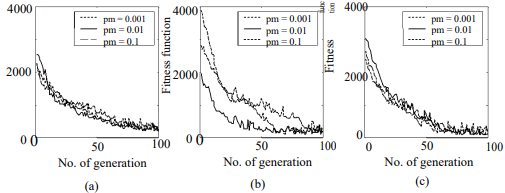
\includegraphics[width=14.0cm, height=4.0cm]{Extras/fig1.png}
         \caption{Sample of Figure/Graph}
         \label{fig:1}
\end{figure*}

\section{Sample of Equation in Text}
The feature that makes LATEX the right editing tool for scientific documents is the ability to render complex mathematical expressions. This article explains the basic commands to display equations.
\begin{equation}
  f(x) \&= x^2
\end{equation}
LaTeX is a programming language that can be used for writing and typesetting documents. It is especially useful to write mathematical notation such as equations and formulae.

\begin{equation}
 E= mc^2
\end{equation}